\section{Grundlagen}
\label{sec:Grundlagen}
Das Simulieren mit Simscape ermöglicht es, verschiedene physikalische Netzwerke miteinander zu verbinden. So kann das Zusammenspiel der verschiedenen Domänen ausgewertet werden.

\subsection{Aufgabenstellung}
\label{subsec:Aufgabenstellung}
Die Aufgabe besteht darin, einen beheizten Swimmingpool zu modellieren und zu simulieren. Dabei sollen das Aufheizverhalten sowie der stationäre Zustand untersucht werden. Als Vorlage wird ein bestehender Pool verwendet. Die Abmessungen werden übernommen, sodass die Resultate der Simulation mit den Temperaturwerten des Pools verglichen werden können.

Die Simulation wird jedoch ein wenig vereinfacht. So werden nicht wie in echt fünf kleine Düsen, sondern nur eine Zuleitung simuliert. Des Weiteren wird die abgerundete Treppe weggelassen, damit nur ein Quader modelliert werden muss.

\subsection{Annahmen}
\label{subsec:Annahmen}
Damit eine möglichst realistische Simulation durchgeführt werden kann, wird der bestehende Pool mit dem Simscape-Modell angenähert. Um den komplexen Vorgang der Natur beschreiben zu können, werden dabei die folgenden Annahmen und Vereinfachungen getroffen:

\begin{table}[H]
	\centering
	\renewcommand{\arraystretch}{1.2}
	\begin{tabular}{l|l}
		\textbf{Pool / Umgebung}     & \textbf{Annahme}                         \\ \hline
		Länge                        & 8.1\,m                                   \\
		Breite                       & 4\,m                                     \\
		Tiefe                        & 1.5\,m                                   \\
		Solltemperatur vom Pool      & 30\,°C                                   \\
		Hysterese der Reglung		 & 1\,°C                                    \\
		Lufttemperatur      		 & 8\,°C bis 19\,°C                         \\
		Funktion der Lufttemperatur  & Sinus                                    \\
		Bodentemperatur              & Mittelwert der Lufttemperatur $\pm$1\,°C \\
		Funktion der Bodentemperatur & Sinus, 3\,h verzögert gegenüber der Luft \\
		Luftfeuchtigkeit             & 50\,\%                                   \\
		Sonne                        & Täglich 12\,h                            \\
		Funktion der Sonne           & Kosinus-Quadrat                          \\
		Strahlungsaustausch			 & Vernachlässigbar						    \\
		Wind						 & Konstant, sehr schwach
	\end{tabular}
\end{table}

Beim Pool, welcher als Vorlage dient, ist eine Wärmepumpe installiert. Diese erzeugt eine Temperaturdifferenz von 3\,K. Mit einem Volumenstrom von $1013\,^{\si{\ell}}\!/_{\si{h}}$ erreicht man, dass der vorgegebene Pool eine Umwälzzeit von genau zwei Tagen besitzt. Das ergibt eine Heizleistung von

\begin{equation}
	P = c_\text{w} \cdot \Delta T_\text{w} \cdot Q = 4'184\,\frac{\si{J}}{\si{kg} \cdot \si{K}} \cdot 3\,\si{K} \cdot 1'013\,^{\si{\ell}}\!/_{\si{h}} = 3.53\,\si{kW}\,.
	\label{eq:Energie Wärmepumpe}
\end{equation}

Der simulierte Pool wird deshalb mit einer Leistung von 3.53\,kW geheizt.

\newpage
Folgende Literaturwerte werden für die Berechnungen in MATLAB verwendet:

\begin{table}[H]
	\centering
	\renewcommand{\arraystretch}{1.2}
	\begin{tabular}{l|l|lc}
		 & \textbf{Symbol}											& \multicolumn{2}{l}{\textbf{Wert}}	\\ \hline
		\textbf{Spezifische Wärmekapazität}						& $c_{\si{w}}$ 		& 4'184\,$\si{J}/(\si{kg}\cdot \si{K})$ 		& \cite{Wassereigenschaften} 	\\
		\textbf{Verdampfungswärme}								& $q_{\si{w}}$ 		& 2'257\,$kJ/kg$ 							& \cite{Wassereigenschaften} 	\\
		\textbf{Wärmeübergangskoeffizient Wasser zu Luft}			& $h_{\si{Pool, Air}}$ & 8\,$\si{W}/(\si{m}^2\cdot \si{K})$		& \cite{Waermeuebergang}		\\
		\textbf{Wärmewiderstand Boden} 					& $Rth_{\si{G}}$ 		& 2\,$(\si{m}^2\cdot \si{K})/\si{W}$		& \cite{Betonwiderstand}		\\
		\textbf{Absorptionskoeffizient} 							& $k$				& 0.1917\,m$^{-1}$							& \cite{Waermekoeffizient}		\\
		\textbf{Sonnenenergie pro Quadratmeter}					& $P_{\si{S, perp}}$	& 1.36\,kW									& \cite{EnergieDerSonne}		\\
		\textbf{Wasserverdunstung pro Quadratmeter und Tag}	& $m_{\si{ev}}$		& 2.27\,kg 									& \cite{WasserVerdunsten}
	\end{tabular}
\end{table}

Abbildung \ref{fig:umgebung} zeigt die Kurvenformen der verschiedenen Umgebungseinflüsse:

\begin{figure}[H]
	\centering
	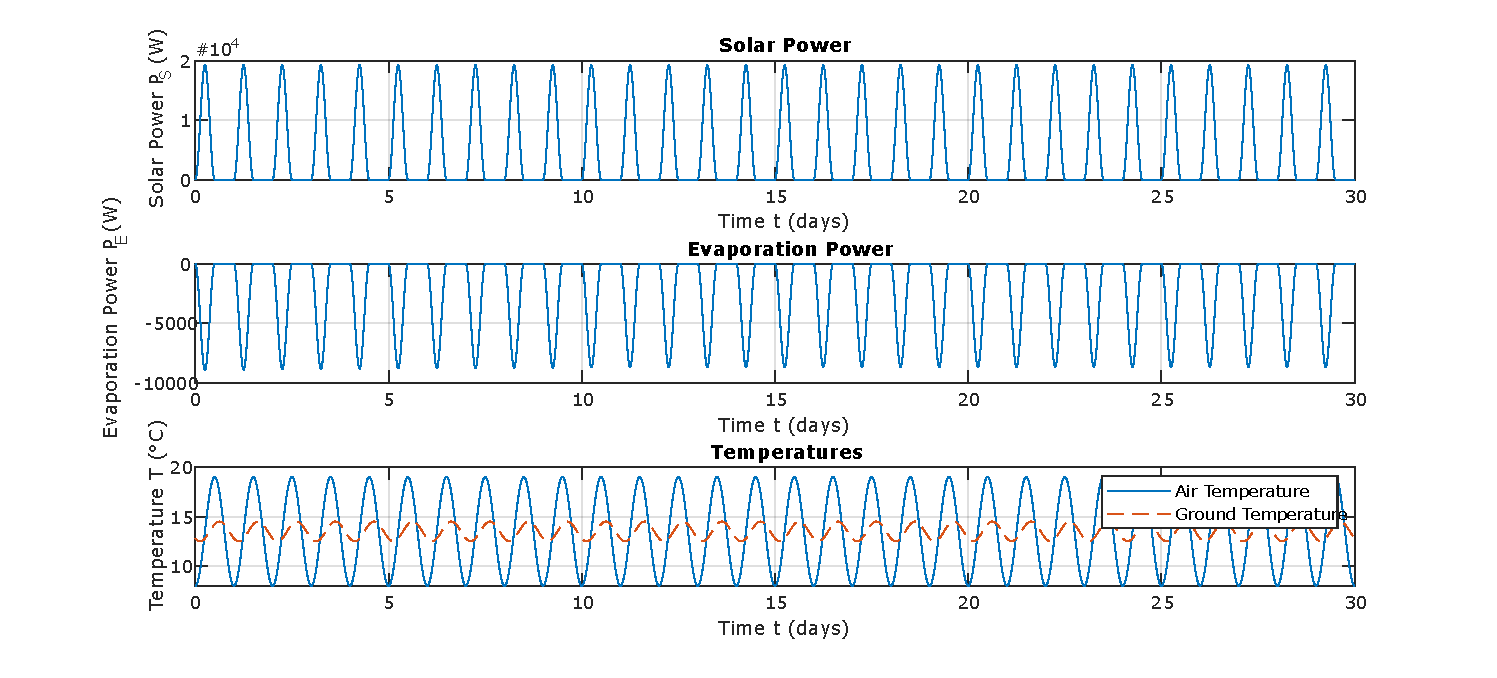
\includegraphics[width=\linewidth]{umgebung}
	\caption{Kurvenformen der Umgebungseinflüsse}
	\label{fig:umgebung}
\end{figure}
